\newpage
\subsection*{\underline{WKB Approximation}}

\begin{align}
	\psi(x) \approx \frac{C}{\sqrt{p(x)}} \, e^{\pm \frac{i}{\hbar} \int p(x)\, dx}
	\qquad \psi(x) \approx \frac{C}{\sqrt{|p(x)|}} \, e^{\pm \frac{i}{\hbar} \int |p(x)|\, dx}; \quad E < V
\end{align}
\begin{align}
	T \sim e^{-2 \gamma}, \qquad \gamma \equiv \frac{1}{\hbar} \int_0^a |p(x)|\, dx
\end{align}
\begin{align}
	\psi(x) \approx \begin{cases}
		\frac{2D}{\sqrt{p(x)}} \sin{\left[ \frac{1}{\hbar} \int_{x}^{x_2} |p(x')|\, dx' \right]}, & x<x_2 ; \\
		\frac{D}{\sqrt{|p(x)|}} \exp{\left[- \frac{1}{\hbar} \int_{x_2}^x |p(x')|\, dx' \right]}, & x>x_2.
	\end{cases}
\end{align}
Potential well with two vertical walls
\begin{align}
	\int_0^a p(x) \, dx
\end{align}
Potential well with one vertical wall
\begin{align}
	\int_0^{x_2} p(x)\, dx = \left(n - \frac{1}{4} \right) \pi \hbar
\end{align}
Potential well with no vertical walls
\begin{align}
	\int_{x_1}^{x_2} p(x) \, dx = \left( n - \frac{1}{2} \right) \pi \hbar
\end{align}

\begin{wrapfigure}{r}{0.95\linewidth}
	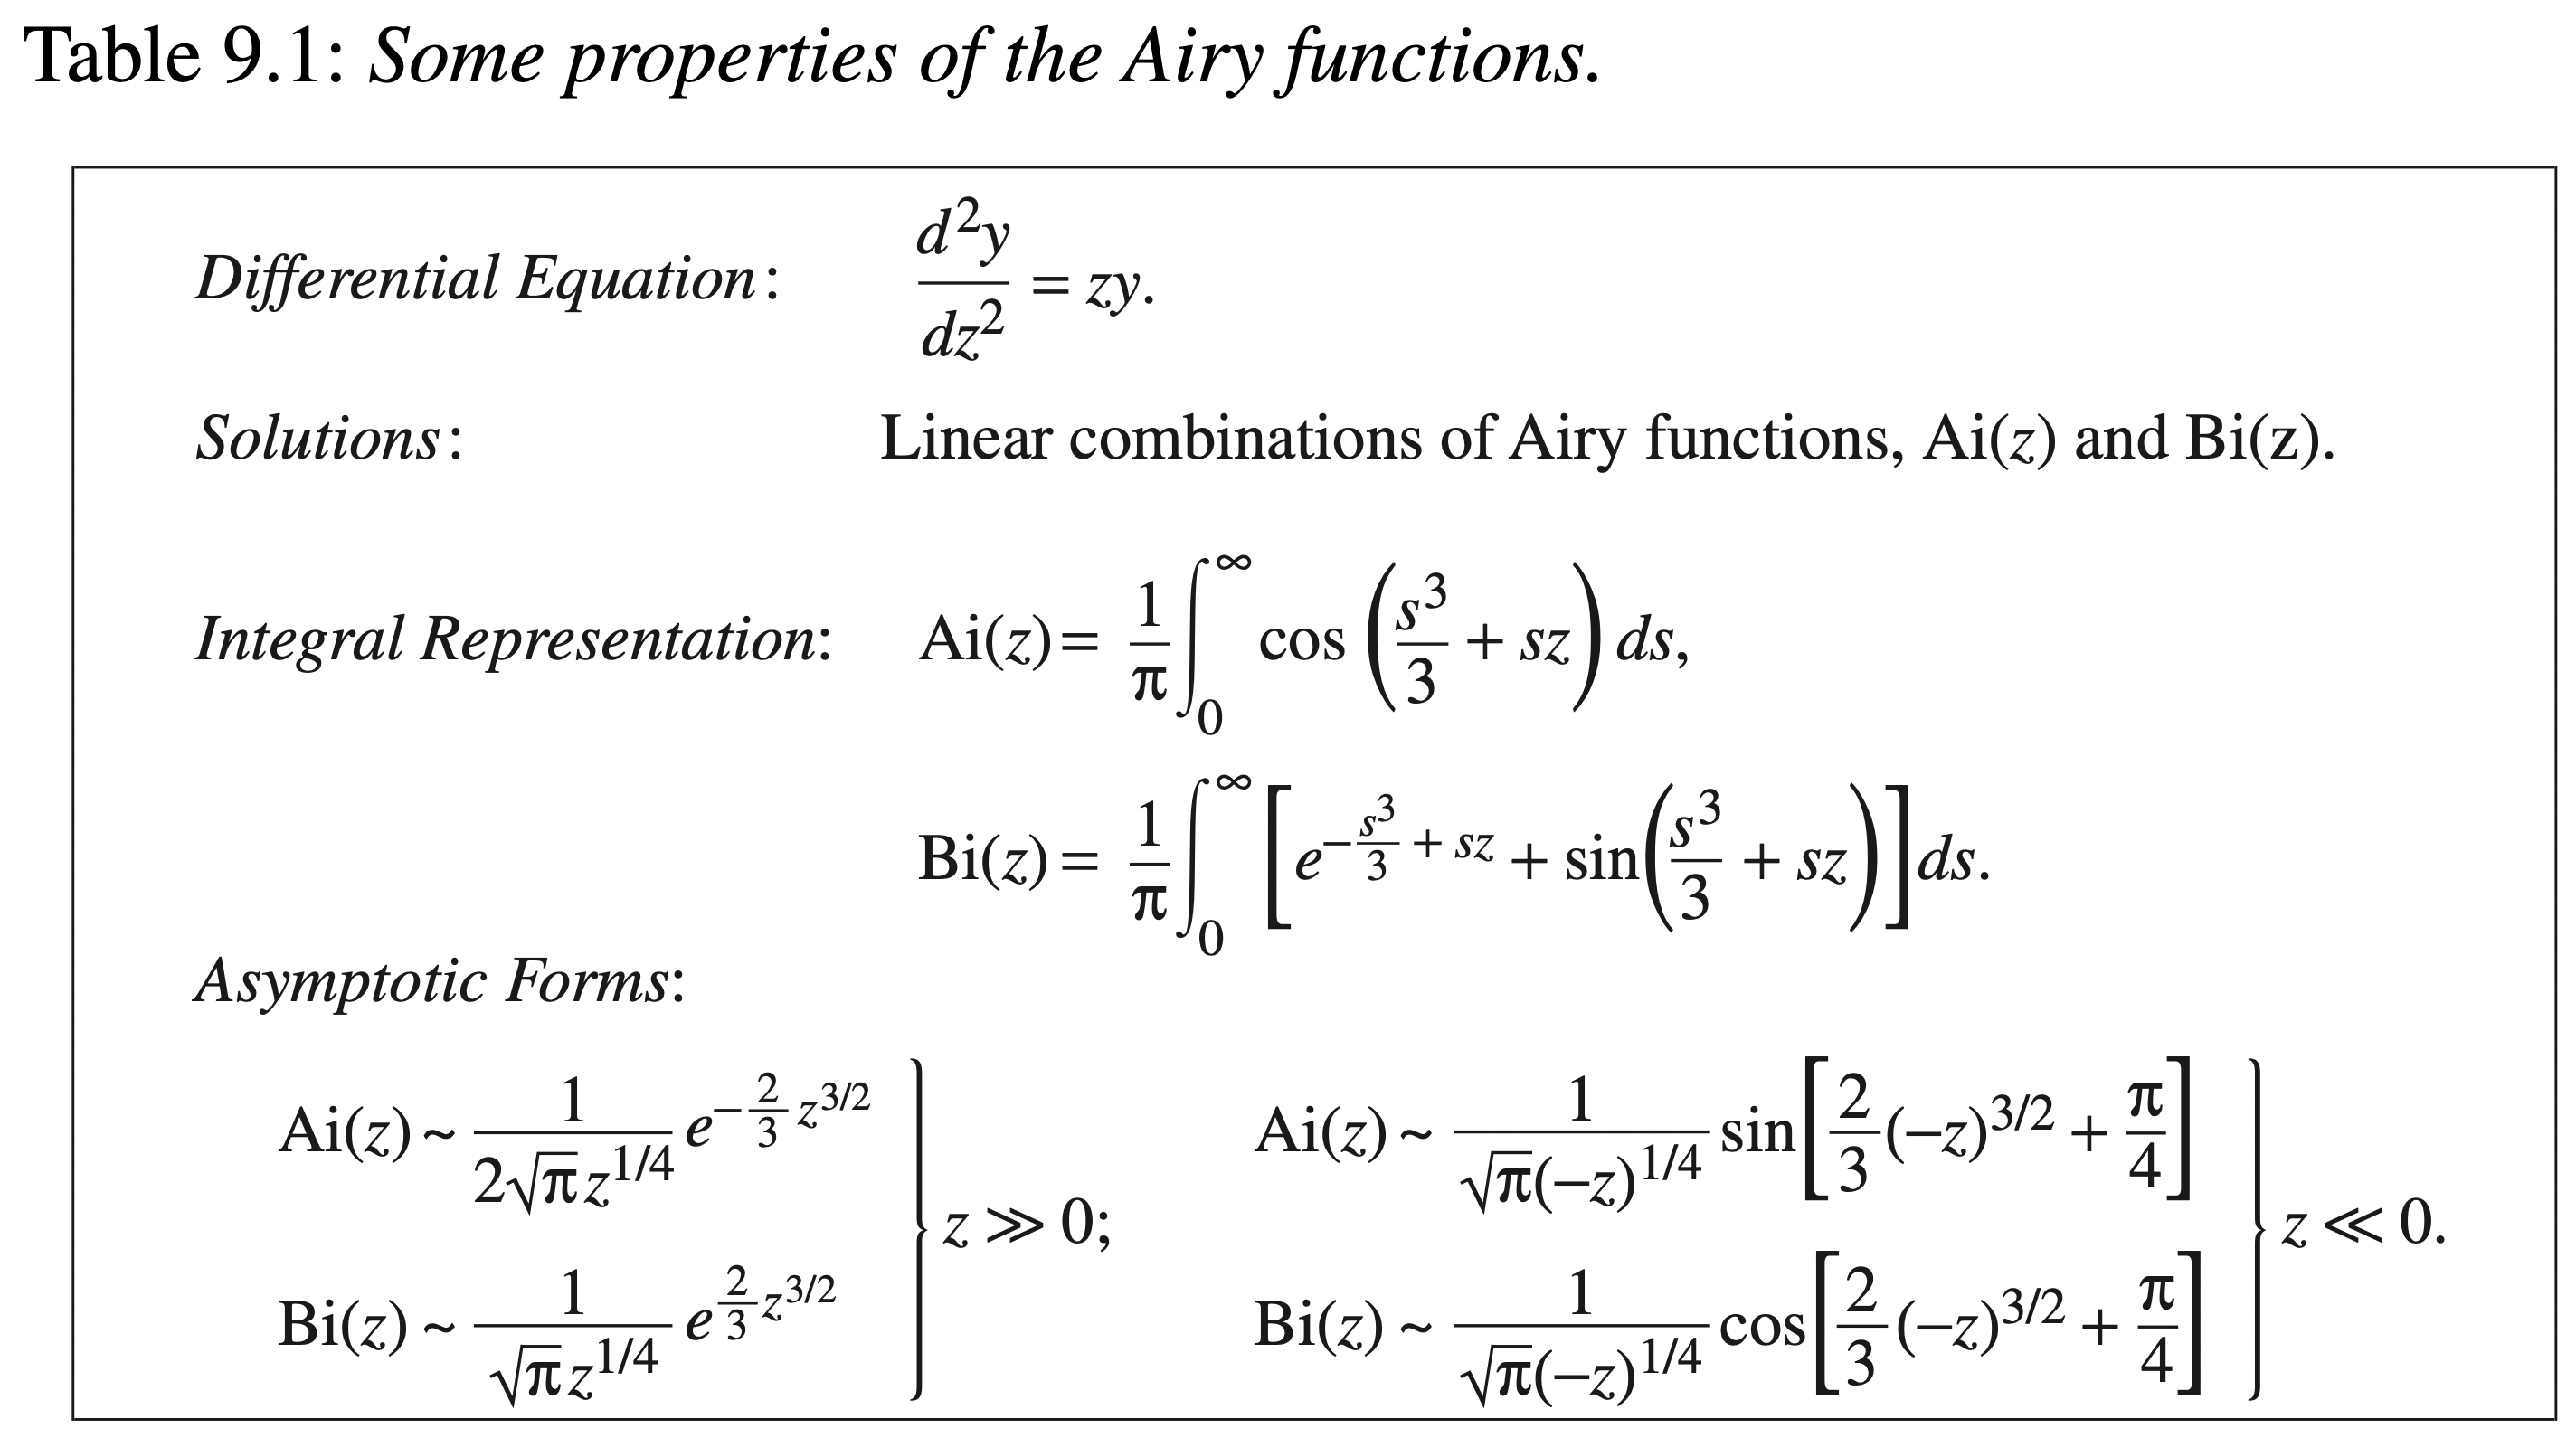
\includegraphics[width=1\linewidth]{./figures/Airy.png}
	\label{fig:Airy properties}
\end{wrapfigure}
